\documentclass[10pt]{article} 
 \usepackage[hang,small,bf]{caption}    % fancy captions
 \usepackage{tikz}	

% TikZ libraries 
\usetikzlibrary{shapes,snakes} 
\usetikzlibrary{backgrounds,fit,decorations.pathreplacing} 
 \usetikzlibrary{shapes,arrows,fit,calc,positioning,automata} 
\newcommand{\ket}[1]{\ensuremath{\left|#1\right\rangle}} % Dirac Kets 
\begin{document} 
    \begin{figure} 
    \centerline{ 
        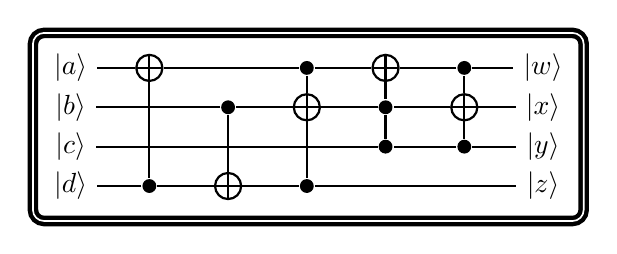
\begin{tikzpicture}[framed,background rectangle/.style={double,ultra thick,draw,rounded corners},thick] 
            \tikzset{oplus/.style={path picture={% 
            \draw[black] 
            (path picture bounding box.south) -- (path picture bounding box.north) 
            (path picture bounding box.west) -- (path picture bounding box.east);
            }}}
             \tikzstyle{operator} = [draw,fill=white,minimum size=1.5em] 
             \tikzstyle{phase} = [fill,shape=circle,minimum size=5pt,inner sep=0pt]
             \tikzstyle{surround} = [fill=blue!10,thick,draw=black,rounded corners=2mm]
             \tikzstyle{swap} = [draw,fill,shape=cross out,minimum size=5pt,inner sep=0pt]
             \tikzstyle{cnot} = [oplus,draw,thick,circle]		% Qubit
		\node at (0,-0.0)(q0_0) {\ket{a}};
		\node at (0,-0.5)(q0_1) {\ket{b}};
		\node at (0,-1.0)(q0_2) {\ket{c}};
		\node at (0,-1.5)(q0_3) {\ket{d}};
		% Gate 1
		\node[phase] (q1_3) at (1,-1.5) {} edge [-] (q0_3);
		\node[cnot] (q1_0) at (1,-0.0) {} edge [-] (q0_0);
		\draw[-] (q1_0)  -- (q1_3);
		% Gate 2
		\node[phase] (q2_1) at (2,-0.5) {} edge [-] (q0_1);
		\node[cnot] (q2_3) at (2,-1.5) {} edge [-] (q1_3);
		\draw[-] (q2_1)  -- (q2_3);
		% Gate 3
		\node[phase] (q3_0) at (3,-0.0) {} edge [-] (q1_0);
		\node[phase] (q3_3) at (3,-1.5) {} edge [-] (q2_3);
		\node[cnot] (q3_1) at (3,-0.5) {} edge [-] (q2_1);
		\draw[-] (q3_0)  -- (q3_1);
		\draw[-] (q3_1)  -- (q3_3);
		% Gate 4
		\node[phase] (q4_2) at (4,-1.0) {} edge [-] (q0_2);
		\node[phase] (q4_1) at (4,-0.5) {} edge [-] (q3_1);
		\node[cnot] (q4_0) at (4,-0.0) {} edge [-] (q3_0);
		\draw[-] (q4_0)  -- (q4_1);
		\draw[-] (q4_1)  -- (q4_2);
		% Gate 5
		\node[phase] (q5_0) at (5,-0.0) {} edge [-] (q4_0);
		\node[phase] (q5_2) at (5,-1.0) {} edge [-] (q4_2);
		\node[cnot] (q5_1) at (5,-0.5) {} edge [-] (q4_1);
		\draw[-] (q5_0)  -- (q5_1);
		\draw[-] (q5_1)  -- (q5_2);
		% Output
		\node at (6,-0.0)(q6_0) {\ket{w}};
		\draw[-] (q5_0)  -- (q6_0);
		\node at (6,-0.5)(q6_1) {\ket{x}};
		\draw[-] (q5_1)  -- (q6_1);
		\node at (6,-1.0)(q6_2) {\ket{y}};
		\draw[-] (q5_2)  -- (q6_2);
		\node at (6,-1.5)(q6_3) {\ket{z}};
		\draw[-] (q3_3)  -- (q6_3);
		\end{tikzpicture} 
   }
\end{figure}
\end{document}
